\documentclass[10pt, letterpaper]{article}
% !TeX root =../main.tex
% !TeX spellcheck = en_US

\usepackage[in]{fullpage}
\usepackage{hyperref}
\usepackage[utf8]{inputenc}
\usepackage[numbers]{natbib}
\usepackage{doi}
\usepackage[affil-it]{authblk}
\usepackage{xspace}
\usepackage{amssymb}
\usepackage{amsmath}
\allowdisplaybreaks
\usepackage[numbers]{natbib}
\usepackage[utf8]{inputenc}
\usepackage[T1]{fontenc}
\usepackage[USenglish ]{babel}
\usepackage{url}
\usepackage{enumerate}
\usepackage{paralist}
\usepackage{here}
\usepackage[textsize=footnotesize]{todonotes}
\usepackage{doi}
\usepackage{xspace}
\usepackage{lipsum}

\usepackage{multirow}
\usepackage{siunitx}
\sisetup{locale = US}
\DeclareSIUnit{\mph}{mph}


\usepackage{tikz}
\usepackage{xcolor}
\usetikzlibrary{shapes}

% !TeX root =../main.tex
% !TeX spellcheck = en_US

\xspaceaddexceptions{())]\}}
\newcommand{\VRPTW}{VRPTW\xspace}



\title{DRAFT \\
Bridge Capacities
}
%Finding the optimal fleet size and mix for
%grocery home delivery services
% \footnote{This work was supported by Lakeside Labs GmbH, Klagenfurt, Austria and funding from the European
% Regional Development Fund and the Carinthian Economic Promotion Fund (KWF) under grant 20214/31942/45906.}
% }

\author[1]{Christian Wankm\"uller}

\author[2] {Christian Truden}
\author[3]{Andreas Felsberger}
% \affil[1]{Department of Mathematics, Alpen-Adria-Universit\"at Klagenfurt, Klagenfurt, Austria.}
\affil[1,3]{Department of Operations Management and Logistics, Alpen-Adria-Universität Klagenfurt,
Klagenfurt, Austria}
\affil[2]{Lakeside Labs, Klagenfurt, Austria}



\begin{document}

\maketitle

\begin{abstract}
  % !TeX root =./main.tex
% !TeX spellcheck = en_US

The transportation of oversize and heavyweight cargoes (OHC) represents one of the most challenging processes in freight movement, frequently leading to time-consuming and costly road closures, traffic congestions and temporary adaptations of infrastructure. In recent years, OHC transportation is gaining massive momentum due to an increasing economic development, general technological progress, and the growing prevalence of large-scale facilities such as wind mills or power plants. Apart from cost and time-related factors, security and safety issues have top priority when undertaking OHC transports on the road. Planning such transports is a complex task due to a multitude of criteria that need to be evaluated before determining the final route. In addition to physical road characteristics, road turning radius and transport corridor widths, the maximum bridge carrying capacity is an important safety-relevant parameter that highly influences OHC transports. Critical incidents, such as the Genoa bridge collapse in 2018, are negative examples where poor maintenance coincides with planning insufficiencies and non-compliance to standards and regulations. In this study, we take up the problem of selecting the optimal route for OHC transports under certain restrictions. In doing so, we propose an integer linear model with the objective to minimize road distance while considering maximum bridge carrying capacities. We test the model to balance cost, time and safety of OHC transportation using data of the Austrian highway network.

\end{abstract}
\noindent%
{\it Keywords: Attended Home Delivery, Fleet Size, Tactical Planning}


\section{Introduction}
\label{sec:intro}
  % !TeX root =./main.tex
% !TeX spellcheck = en_US

Due to the global economic expansion, the transport sector has been gaining massive momentum for years.
Since 2010, global freight volumes continuously increase with forecasts predicting growth rates of 3.2\% per year until 2050 \cite{figura2020preferences, InternationalTransportForum}.
Various transportation modes, including rail, maritime, air, and road, are available to cope with this rapid development and to satisfy future transportation needs.
However, primary focus is generally placed on the road transport segment due to its dominating role for domestic transportation, with almost 80\% of the total volume of goods being carried by trucks in the European Union \cite{Eurostat}.
The increase in demand for transportation also holds true for superheavy, bulky and extra-large goods \cite{gavrilova2021analysis}, referred to as oversized and heavyweight cargoes (OHC) in this article \cite{Luo.2021}.
OHC is typically associated with the transportation of industry goods (e.g. generators, turbines, construction equipment) that exceed maximum legal limits in terms of weight and/or size.
In comparison with traditional freight transportation, OHC often requires time-consuming and complex efforts with regard to the planning and execution, as no two OHC transports are completely the same \cite{Wolnowska.2019}.
Some OHC transports may require complete road closures or detours and the escort by police and other law enforcement.
Consequently, the planning is usually conducted on an individual level, taking the different specifications of each OHC into consideration \cite{Bazaras.2013}.
Here, several relevant technical, administrative and organizational criteria are subject of detailed analysis to reduce technical, economic, social and political risks, thereby increasing the safety of OHC transports \cite{Palsaitis.2012}.
Granular planning is further dependent on national standards and legislations. Due to legal requirements, it generally involves the evaluation of multiple factors related to restrictions in terms of physical characteristics of roads, road turning radius, total length of the route, demand for installation of transshipment sites or obstacles along the road \cite{PETRASKA.2018}.
Especially, oversized load is limited by road turning radius, transport corridor width and road-side obstacles, such as traffic lights or power lines.
Hence, planning is dominated by local characteristics and in-person inspection is required once a particular transport route has been submitted to the authority.
Overweight load, i.e. vehicles loaded with more than 11 tons per axle, are even more difficult to plan than over-sized load.
One of the most safety-relevant attributes that needs to be considered in this respect is the maximum bridge carrying capacity, which must not be surpassed by the total weight of a OHC transport, and thus, is highly influencing route planning activity.
This is for two reasons; excessive overload significantly contributes to shorten service lifes of pavements and bridges; and reduces bridge safety to levels that may fall below those set in the design standards, potentially resulting in failures or collapse \cite{fiorillo2018fragility}.
Critical incidents, such as the Genova bridge collapse in 2018 \cite{Morgese.2020, MorandiNYTimes},  demonstrate the effects of long-term exceeding of permitted limits on infrastructure, thereby underlining the importance of complying with certain standards and norms in OHC planning.

\par In practice, the route planning process for oversize and heavyweight transports involves several stakeholders, such as client companies, carriers, governmental institutions and civil engineers.
This labor intense planning procedure is described in \cite{Osegueda.1999}. In the beginning, the client company or carrier drafts a first route design and submits this draft to the responsible authority for approval.
Subsequently, a civil engineer is consulted who determines the maximum allowable weight and speed on every single bridge of the proposed route.
Aside from statical calculations, the civil engineer relies on on-site visits and inspections of bridge elements to evaluate their tolerances, technical specifications, and other structural parameters.
In case of route infeasibility due to exceeding of permitted limits or necessary changes for any other reason, the initial draft needs to be revised, adapted, and resubmitted by the applicant and subsequently re-evaluated by the civil engineer.
This costly and time-consuming process must be repeated until the route is declared feasible and a permit is granted.
What seems to be problematic in this respect is that the development of the initial draft is primarily based on commercial GIS applications that are limited in terms of data availability and accuracy.
Standard GIS solutions indeed consider temporary construction sites or road closures but exhibit a severe lack of data on bridge locations and the respective bridge carrying capacities, and thus, do not facilitate the identification of an optimal route under consideration of weight limits.
Therefore, there is a need of professional software that thoroughly takes weight parameters into account.
\par In an attempt to simplify the cumbersome authorization process, we take an optimization approach.
To this end, a mathematical model is used to determine the optimal path between two points within the road network while respecting certain constraints, i.e., weight limits, for example.
Under the assumption that the model results in more than one feasible routes, a study that compares several (possibly conflicting) objectives will be conducted.
In doing so, we consider different types of vehicles and loads. The results should provide \textit{decision support} for reducing the complexity of OHC route planning. 
\par
The article continues with a review of the existing body of knowledge in the respective field (Section 2).
Then, we provide the problem description and introduce notations along with the model assumptions in section 3. Next, the optimization model is presented and illustrated in an example of application (Section 4).
Finally, section 5 closes the article, summarizing the research implications, study limitations and future lines of research.



\section{Related Work}\label{sec:related}
%
% !TeX root =./main.tex
% !TeX spellcheck = en_US

Increasing economic development, general technological progress, and the growing prevalence of large-scale facilities, such as wind mills or power plants, increase the demand for OHC transports.
Frequently, these transport processes are executed within the road network. This is because roads exhibit a high geographical coverage and thus, provide a certain amount of flexibility and cost saving potential, as goods can often be delivered directly without any time-consuming handling or transshipment efforts being required. However, taking into account the complexity of road transportation as well as the potential damage caused to pavements and bridges, OHC route selection is a highly challenging task \cite{Bazaras.2013, xu2001methodology, sivilevicius2007dynamics, fiorillo2016minimizing}. Yet, selection of an optimal route based on reasonable route planning methods greatly improves the efficiency of OHC transports \cite{meng2015optimized}.
Therefore, optimal route selection in the field of road-related OHC has recently become a topic of considerable relevance \cite{geisberger2011efficient, yan2018optimal}.
\par
This paper is building upon past research on OHC routing. In the literature, a wide range of different approaches to this issue are presented. Fu and Hag-Elsafi \cite{fu2000vehicular}, for example, address the overload monitoring and permitting procedure. In doing so, reliability models for assessing bridge safety are described. Moreover, permit-load factors for monitoring purposes are proposed. Ghosn, in turn, focuses on truck weight regulations and the corresponding bridge safety levels using reliability indices \cite{ghosn2000development}. Vigh and Kollár, again, elaborate on methods that take into account different bridge structures as well as vehicle and loading characteristics in the permitting process \cite{vigh2006approximate, vigh2007routing}
\par
One particular method for optimal route selection is the integration and processing of all available data concerning the road network in a Geographic Information System (GIS) \cite{durham2002gis}.
According to Datla et al. \cite{datla2004gis}, a GIS facilitates identification of shortest paths, while taking into account characteristics and attributes of the road network as well as the involved transport vehicles, provided that data are available and up-to-date. Relevant parameters, such as vehicles' load, height, width, weight, and weight distribution, are considered to take into account restrictions, ensuring safety, and preventing damage to infrastructure elements such as bridges \cite{ecmt2006improving, vaitkus2016effect, kombe2017modelling, pauer2017development}. According to Adams et al. \cite{adams2002enterprise}, a GIS-based system also facilitates the automation of the permission process by considering spatial and temporal constraints during the path-finding process, given that the respective systems for routing and authorization purposes are well integrated. However, the authors also emphasize the difficulty of aligning enterprise databases of bridges and highways with the requirements of GIS-based permitting systems, which is frequently resulting in severe data management problems.
\par
According to Bazaras et al. \cite{Bazaras.2013}, safety, security, and reliability are indeed three very important aspects that have to be considered to increase the overall quality of transport processes. Therefore, apart from regular driving training and state-of-the-art equipment, detailed risk evaluation is regarded to be a key issue in terms of OHC routing. The authors also underline that a fuzzy multi-criteria decision making tool is beneficial in the course of route selection, as it allows taking into account the variety of influencing factors. Apart from road quality, turning radius, corridor widths and heights, bridge carrying capacities, reloading and storing opportunities, regular traffic intensity on route segments, and seasonal specialties, a multi-criteria system might also include an assessment of required road texture improvements and other structural adaptations or changes.
\par
In summary, the respective literature does not take adequate account of bridge carrying capacities as an important influencing factor for OHC route selection. We assume the underlying reason being a general lack of data and insufficient data quality on exact bridge locations and carrying capacities.



% \begin{itemize}
%
%   \item Commercial Solutions
%
%   \item HERE
%   \url{https://www.here.com/}
%   \item PRISMA
%   \url{https://www.prisma-solutions.com/}
%
%   \item Bentley Superload Routing
%   \url{https://www.bentley.com/en/products/product-line/asset-performance/superload-routing}
%
% \end{itemize}


\section{Model}\label{sec:model}
%
% !TeX root =./main.tex
% !TeX spellcheck = en_US


\subsubsection{Transport Request}

A \emph{transport request} $r=(o,d,w,g) \in \mathcal{V} \times \mathcal{V} \times \mathbb{R}^{+}$
has an \emph{origin} $s$, a \emph{destination} $t$, a \emph{total weight} $w$, and
a \emph{maximal gradient} $g$.
The maximal gradient defines which climbs or descent can be done with the transport in a safely manner.

\subsubsection{Matrix Representation of the Road Network}

The vertices of the matrix are the crossing points of the roads, while
the road section connecting those points form the edges of the matrix.
For each edge, we have the distance between the vertices and the length of the bridges along the segment
and the capacity constraints (and the lowest encountered bridge capacity).
This way, we can answer various questions concerning transports between those vertices.
Without loss of generality, we assume an undirected graph.
In that sense, the travel distance along an edge is independent of
the travel direction, and  the same bridges are surpassed in both directions.
The problem statement can
easily be extended to a directed graph. However, the authors omitted this for reasons of simplicity.

Classically,  the considered network $\mathcal{N}=(\mathcal{V},\mathcal{E})$ consists of
\begin{itemize}
  \item \emph{Nodes} (vertices) $\mathcal{V}=\{1,\ldots, n\}$, which represent the intersections of the road segments,
as  well as the start (end) points of the roads, and

  \item \emph{Links} (edges) $\mathcal{E} \subseteq \mathcal{L} \times \mathcal{L}$,
  correspond to the roads (road segments) connecting the vertices \cite{liedtke2012generation}.
\end{itemize}

Road links $e \in \mathcal{E}$ have a length $\ell(e)\in \mathbb{R}^{+}$ representing their road length.
Further, they have a weights $c(e) \in C$ giving their \emph{classification} following \textit{Open Street Map} (OSM) \cite{OpenStreetMap}. Starting from the highest level, we classify the roads
$C=\{0,1,2\,\ldots\}$ where these are regarded dimensionless units.

For each road link  $e \in \mathcal{E}$ we know the \emph{maximum gradient} $g(e) \in [0,1)$ which gives the steepest ascending or descending gradient (measured in percent).

Bridges (and other types of building structures that must be overpassed)
have \emph{weight limits} (measured in metric tons) which are determined by civil engineers.
Each road link $e \in \mathcal{E}$ contains a nonnegative number of bridges, where each has a weight limit.
For each link $e$, we set a \emph{weight limit} $w(e) \in \mathbb{R}^{+}$ which is the
minimum over all bridges on this link and the \emph{number of bridges} $b(e) \in \mathbb{N}^{0}$.
A weight limit $w(e)= \infty$ describes the circumstance
that no limit is given for $e$.

A simple toy example, see Figure \ref{fig_toy_example_1}, shall illustrate these definitions.
\begin{figure}[!ht]
  \centering
  % !TeX root =../main.tex
% !TeX spellcheck = en_US



% https://tex.stackexchange.com/questions/64252/tikz-midway-label-on-a-bended-line
% https://texample.net/tikz/examples/p2p-topology/

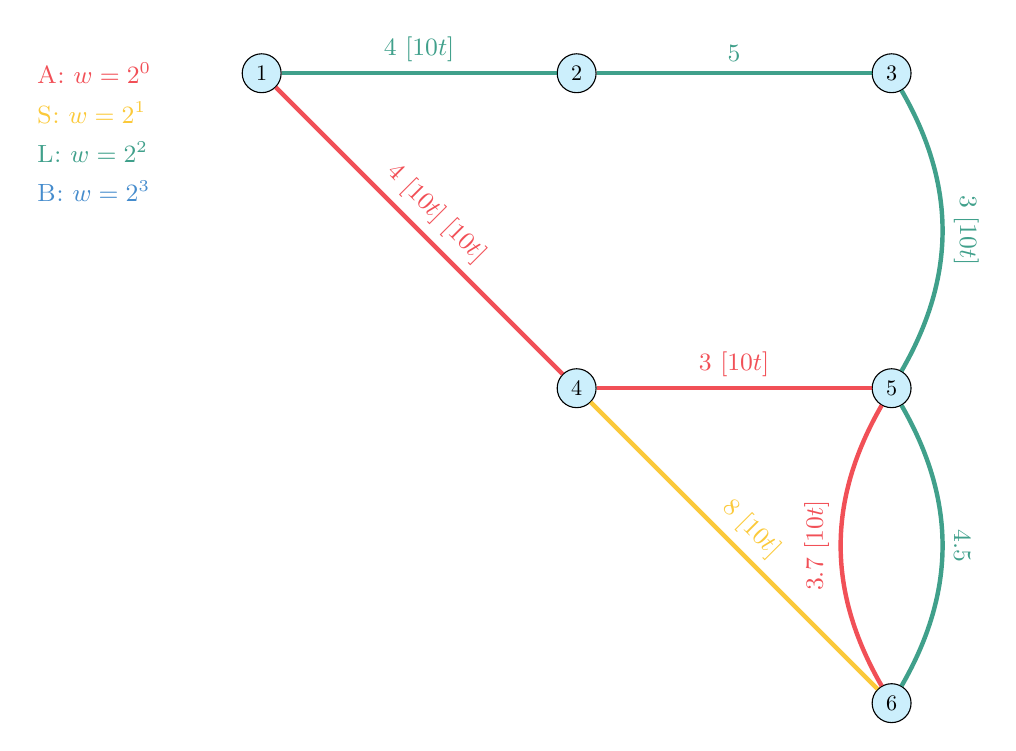
\begin{tikzpicture}[auto, thick]

  % Define Colors
  \definecolor{pinegreen}{cmyk}{0.92,0,0.59,0.25}
  \definecolor{royalblue}{cmyk}{1,0.50,0,0}
  \definecolor{lavander}{cmyk}{0,0.48,0,0}
  \definecolor{violet}{cmyk}{0.79,0.88,0,0}
  \definecolor{red}{cmyk}{0,0.95,0.90,0}
  \definecolor{yellow}{cmyk}{0,0.25,1,0}

  % Node styles
  \tikzstyle{cblue}=[circle, draw, thin,fill=cyan!20, scale=0.8]
  \tikzstyle{qgre}=[rectangle, draw, thin,fill=green!20, scale=0.8]

  \tikzstyle{A_path}=[ultra thick, red, opacity=0.8, font=\small]
  \tikzstyle{S_path}=[ultra thick, yellow, opacity=0.8, font=\small]
  \tikzstyle{B_path}=[ultra thick, royalblue, opacity=0.8, font=\small]
  \tikzstyle{L_path}=[ultra thick, pinegreen, opacity=0.8, font=\small]


  % Nodes
  % \node[cblue] (n_1_1) at (0,0) {1};
  % \node[cblue] (n_2_1) at (4,0) {2};
  \node[cblue] (n_6) at (8,0) {6};

  % \node[cblue] (n_1_2) at (0,4) {4};
  \node[cblue] (n_4) at (4,4) {4};
  \node[cblue] (n_5) at (8,4) {5};

  \node[cblue] (n_1) at (0,8) {1};
  \node[cblue] (n_2) at (4,8) {2};
  \node[cblue] (n_3) at (8,8) {3};




  %  A links

  \draw[A_path] (n_4)--  (n_5)  node [midway, above, sloped] (TextNode) {$3~[10t]$};
  \draw[A_path] (n_6) to[bend left]   node [midway, above, sloped]  {$3.7~ [10t]$} (n_5)  ;
  \draw[A_path] (n_4) -- (n_1)  node [midway, above, sloped] (TextNode) {$4 ~[10t]~[10t]$};


  % S links
  \draw[S_path] (n_4) to node [midway, above, sloped] {$8~ [10t]$} (n_6);

  %  L lines
  \draw[L_path] (n_1) --  (n_2)  node [midway, above, sloped] (TextNode) {$4~[10t]$};

  \draw[L_path] (n_2)--  (n_3)  node [midway, above, sloped] (TextNode) {$5$};
  % \draw[L_path] (n_3) to[out=-20,in=-20]  (n_5)  node [midway, above, sloped] (TextNode) {$l=3, b=2$};
  \draw[L_path] (n_3) to[bend left] node [midway, above, sloped]   {$3~[10t]$}    (n_5);


  \draw[L_path] (n_5) to[bend left]  node [midway, above, sloped] {$4.5$} (n_6);

  % B links
  % \draw[B_path] (n_6) to node [midway, above, sloped] {$7; 2$} (n_2_1);


  % Legends
  \node[A_path, anchor=west] at (-3,8){\textsc{A:} $w=2^0$};
  \node[S_path,anchor=west] at (-3, 7.5){\textsc{S:} $w=2^1$};
  \node[L_path,anchor=west] at (-3, 7){\textsc{L:} $w=2^2$};
  \node[B_path,anchor=west] at (-3, 6.5){\textsc{B:} $w=2^3$};

\end{tikzpicture}

  \caption{Toy Example 1.}
  \label{fig_toy_example_1}
\end{figure}


\subsubsection{Feasible Sub-Network}

Clearly, a transport $r$ can only traverse road links $e \in \mathcal{E}$ for which $w(r) \leq w(e)$
 $g(r)\geq g^-(e)$ hold.

Accordingly, we define the sub-network $\mathcal{N}_{\omega}$ that contains only the vertices and edges from $\mathcal{N}$ that have a weight limit larger than $\omega \in \mathbb{R}^{+}$ and
does not violate the maximal gradients.
Hence, for the remainder of this manuscript, we set $\mathcal{N}=\mathcal{N}_{\omega=w(r)}$.
In that sense, a transport request $r$ can not be conducted if $\mathcal{N}_{\omega=w(r)}$ is not
connected between $o$ and $d$.

\paragraph{Example}
We consider a request $r=(o,d,w=20t, g=0.10)$ where $o$ and $d$ are somewhere within the network. A road link $e_1=(o_1,d_1, w=30t, g=-0.08)$  can be traversed as, both, the bridge weight capacities and the gradients are feasible. On the other hand,  a link
$e_2=(o_2,d_2, w=10t, g=-0.12)$ cannot be used as there is at least one bridge
on the link that carries only $10t$ (while the transport has $20t$). Also, there
is a $0.12$ descent ($12\,\%$) that cannot be dealt with in a safely manner as the
transport is cannot handle more than $10\%$ gradient.




\section{Shortest Path Problem}


\subsubsection{Integer Programming Formulation}
In order to give an \emph{Integer Programming} (IP) formulation for we enumerate the
vertices $1,\ldots,|\mathcal{V}|$. We consider a directed graph $G=(\mathcal{V},\mathcal{E})$ that is derived from the network $\mathcal{N}$.
In that sense, the auxiliary variables $x_{ij}$, $(i,j) \in \mathcal{V}$
is set to $1$ if and only if node $j$ is visited directly after node $i$, and to $0$ otherwise.
A standard IP formulation to determine the shortest path between $s$ and $t$ can be given as follows
\begin{align}
  \min \quad &\sum_{(i,j)\in \mathcal{E}}  c_{ij} x_{ij} \label{obj} \\
  \text{s.t.}\quad &
  \sum_{(i,j)\in \delta^{+} (i)} x_{ji} - \sum_{(i,j)\in \delta^{-}(i)} x_{ij} =
  \begin{cases}
    1 \quad& \text{if}~ i=s, \\
    -1 \quad& \text{if}~ i=t \\
    0 \quad&\text{else}
  \end{cases}
  \qquad \forall i \in \mathcal{E}
  \\
  &  \sum_{(i,j)\in \delta^{+} (i)} x_{ij}   x_ {ij} \leq 1     \qquad \forall i \in \mathcal{E}\\
  &  x_{ij} \in \{0,1\}   \qquad \forall (i,j) \in \mathcal{V}
\end{align}
The set of outgoing (ingoing) edges of vertex $i$ is denoted by  $\delta^{+} (i)$  $(\delta^{-} (i))$.


\subsubsection{Objectives}

We consider three different objectives, i.e., different assignment of $c_{ij}$.
\begin{enumerate}
  \item \emph{Classic shortest path}, where $c_{ij}=\ell_{ij}$. \label{obj_short}
  \item \emph{Minimal number of surpassed bridges}, where  $c_{ij}=b_{ij}$.  \label{obj_minBridge}
  \item \emph{Prefer high level roads}, where we assign an exponential weighting to the road classes (in ascending order of preference) $C$, $c_0=2^0,c_1=2^1, \ldots$.  \label{obj_highLevelRoad}
  \item \emph{Avoid steep roads}, exponential weights are assigned, i.e., $c_{ij}=\euler^{g(e)}$.
  \label{obj_steep}
\end{enumerate}


\subsubsection{Related Work on the Shortest Path Problem}

\citet{TACCARI2016122, zhu2014vehicle, Osegueda.1999}

\subsubsection{Solution Procedere}


As the considered objectives use costs which induce no \emph{negative cycles}  on $G$, the problem can be efficiently solved
by polynomial-time algorithms like
\emph{Bellman-Ford's} \cite{Bell1958,Ford1956} or \emph{Dijistra's} \cite{dijkstra1959note} algorithm.
% In case of \ref{obj:obj_minBridge}, links having no bridges ($b(e)=0$) can induce cycles which are of length zero.


% bjectives are:
% \begin{itemize}
%   \item Shortest Path (classic).
%
%   \item Minimal wear of infrastructure. Reducing the wear induced by over-weight transports
%   minimizes maintenance costs, extends lifetime of the building structures, and
%   improves safety (Genoa bridge collapse in 2018).
%   \citet{Kakan2014}
%
%   % \item Minimize the number of different road operators and municipalities the path
%   % traverses. In that sense, the process of getting official approval of the
%   % path should be simplified.
%
%   \item Number of Bridges, i.e., less work for the civil engineer.
%   \item Preferably high level roads (if possible).
%   Achieve this be exponential weightening of the road segments.
%   \textit{A}: $w=2^0$,    \textit{S}: $w=2^1$,      \textit{B}: $w=2^2$,     \textit{L}: $w=2^3$.
%   The considered Austrian road network is clearly structured into these road levels.
%   Clearly, for any other network, a similar weightening be introduced
%   (if not given) under consideration of the road widths etc.
% \end{itemize}
%
% \begin{itemize}


% https://algs4.cs.princeton.edu/44sp/
% https://jgrapht.org/javadoc-SNAPSHOT/org.jgrapht.core/org/jgrapht/alg/shortestpath/DijkstraShortestPath.html


\section{Example of Application and Results}\label{sec:application}
%
% !TeX root =./main.tex
% !TeX spellcheck = en_US
\subsection{Study setting}
The study at hand was conducted as part of the joint Interreg project SWEET (Single Window for Exceptional Transport) with the objective to harmonize cross-border \ohc transportation between Austria and Italy \cite{Sweet}. In detail, the project pursues the goal of developing and implementing a digital platform solution to enable coordinated processing of \ohc related tasks. Here, special interest lies in the streamlining of different national legislations, simplifiening of authorization processes, improving governance and enabling real-time monitoring of transports. The project further fosters the determination of adequate transport corridors and the automatization of optimal route selection as part of the \ohc planning phase. This is where the subsequent study contributes by proposing a robust mathematical approach to provide decision-making support to practicioners.   



% \section{Conclusion}
% \label{sec:concl}
% \input{x_conclusion}

\small
\bibliography{bibliography}
\bibliographystyle{abbrvnat}


\end{document}
